\documentclass{standalone}
\usepackage{graphicx}	
\usepackage{amssymb, amsmath, amsthm}
\usepackage{color}

\usepackage{tikz}
\usetikzlibrary{intersections, backgrounds}

\definecolor{light}{RGB}{220, 188, 188}
\definecolor{mid}{RGB}{185, 124, 124}
\definecolor{dark}{RGB}{143, 39, 39}
\definecolor{highlight}{RGB}{180, 31, 180}
\definecolor{gray10}{gray}{0.1}
\definecolor{gray20}{gray}{0.2}
\definecolor{gray30}{gray}{0.3}
\definecolor{gray40}{gray}{0.4}
\definecolor{gray60}{gray}{0.6}
\definecolor{gray70}{gray}{0.7}
\definecolor{gray80}{gray}{0.8}
\definecolor{gray90}{gray}{0.9}
\definecolor{gray95}{gray}{0.95}

\begin{document}

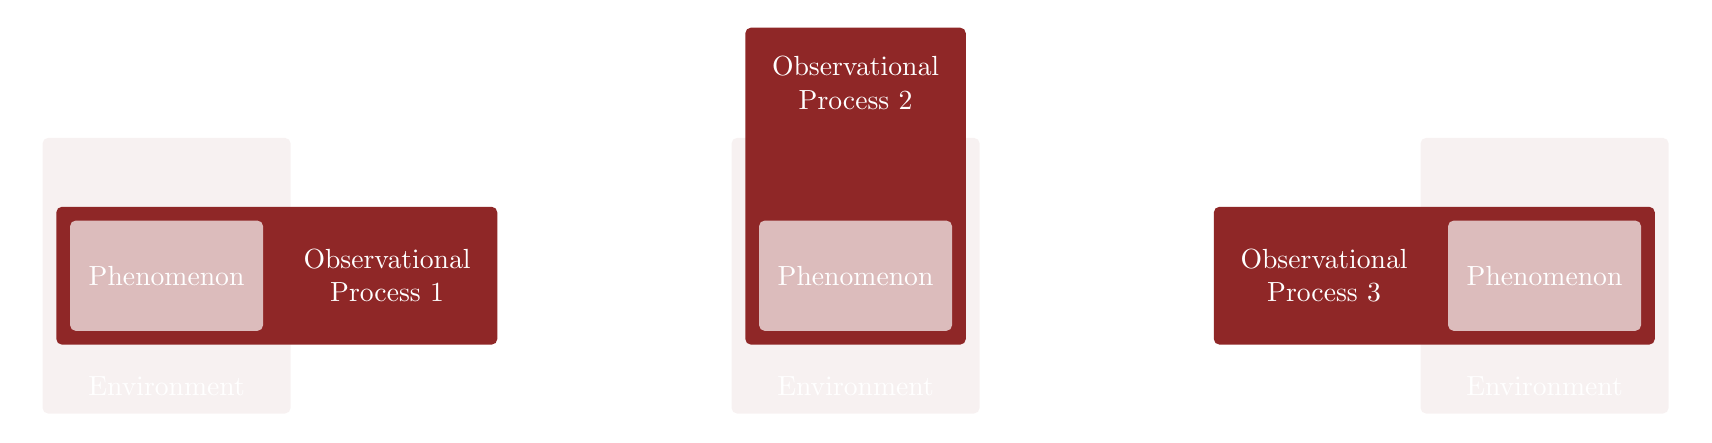
\begin{tikzpicture}[scale=0.35, thick]
  % One
  \pgfmathsetmacro{\dx}{-25}
  
  \filldraw [draw=white, fill=white] (-5 + \dx, -5) rectangle +(17, 13);
  
  \fill [rounded corners=2pt, fill=mid, opacity=0.1] (-4.5 + \dx, -5) rectangle +(9, 10);
  \node at (\dx, -4) [text=white] {Environment};
  
  \fill [rounded corners=2pt, color=dark, dashed] (-4 + \dx, -2.5) rectangle +(16, 5);
  \node at (8 +\dx, 0) [text=white, align=center] {Observational\\Process 1};
  
  \fill [rounded corners=2pt, fill=light, text=white] (-3.5 + \dx, -2) rectangle +(7, 4) 
  node [midway, align=center] {Phenomenon};
  
  % Two
  \pgfmathsetmacro{\dx}{0}
  
  \filldraw [draw=white, fill=white] (-5 + \dx, -5) rectangle +(10, 13);
  
  \fill [rounded corners=2pt, fill=mid, opacity=0.1] (-4.5 + \dx, -5) rectangle +(9, 10);
  \node at (\dx, -4) [text=white] {Environment};
  
  
  \fill [rounded corners=2pt, color=dark, dashed] (-4 + \dx, -2.5) rectangle +(8, 11.5);
  \node at (\dx, 7) [text=white, align=center] {Observational\\Process 2};
  
  \fill [rounded corners=2pt, fill=light, text=white] (-3.5 + \dx, -2) rectangle +(7, 4) 
  node [midway, align=center] {Phenomenon};
  
  % Three
  \pgfmathsetmacro{\dx}{25}
  
  \filldraw [draw=white, fill=white] (-12 + \dx, -5) rectangle +(17, 13);
  
  \fill [rounded corners=2pt, fill=mid, opacity=0.1] (-4.5 + \dx, -5) rectangle +(9, 10);
  \node at (\dx, -4) [text=white] {Environment};
  
  \fill [rounded corners=2pt, color=dark, dashed] (4 + \dx, -2.5) rectangle +(-16, 5);
  \node at (-8 +\dx, 0) [text=white, align=center] {Observational\\Process 3};
  
  \fill [rounded corners=2pt, fill=light, text=white] (-3.5 + \dx, -2) rectangle +(7, 4) 
  node [midway, align=center] {Phenomenon};
  
\end{tikzpicture}

\end{document}  